\documentclass{sig-alternate}

\usepackage{subfigure}

%new package%%%%%%%%%%%%%%%%%%%%%%%
%Danny
\usepackage{multirow}
%%%%%%%%%%%%%%%%%%%%%%%%%%%%%%%%%%%

\sloppy

%--- Code for Shared Affiliations
\def\sharedaffiliation
{
 \end{tabular}
 \begin{tabular}{c}
}
%---

\begin{document}

%--- Start of Table
\begin{table}[t]
\caption{Traffic comparison between IXPs}            
\normalsize                                                          
\centering                                                                  
\begin{tabular}{l|l| r r r r |r r r r| l}                                        
\hline                                                                      
\multirow{2}{*}{\textbf{\begin{tabular}[c]{@{}c@{}}Short \\ Name\end{tabular}}} & 
\multirow{2}{*}{\textbf{Country}} & 
\multicolumn{4}{c}{\textbf{Throughput Maximum (Gbit/s)}} &
\multicolumn{4}{c}{\textbf{Throughput Average (Gbit/s)}} &\\ 

&&\textbf{\begin{tabular}[c]{@{}c@{}}Daily\end{tabular}}& 
\textbf{\begin{tabular}[c]{@{}c@{}}Weekly\end{tabular}}&
\textbf{\begin{tabular}[c]{@{}c@{}}Monthly\end{tabular}}&
\textbf{\begin{tabular}[c]{@{}c@{}}Yearly\end{tabular}}&
\textbf{\begin{tabular}[c]{@{}c@{}}Daily\end{tabular}}&
\textbf{\begin{tabular}[c]{@{}c@{}}Weekly\end{tabular}}&
\textbf{\begin{tabular}[c]{@{}c@{}}Monthly\end{tabular}}&
\textbf{\begin{tabular}[c]{@{}c@{}}Yearly\end{tabular}}&
\\\hline

PTT Metro	& Brazil			&678.50		&698.39		&685.67		&467.46		&393.32		&444.64		&432.21		&360.62 	&(1)\\
AMS-IX		& Netherlands		&3429.38	&-			&-			&3604.48	&2120.70	&-			&-			&1893.38   &(2)\\
MSK-IX		& Russia			&1332.63	&1437.03	&1457.81	&1479.12	&751.24		&796.24		&806.76		&727.27	&(3)\\
DE-CIX		& Germany			&3603.10	&-			&3854.80	&3875.10 	&2375.90	&-			&2299.20	&1964.9  	&(4)\\
LINX		& United Kingdom	&2352.13	&2554.88	&2558.98	&2573.31	&1419.26	&1605.63	&1571.84	&1420.29   &(5)\\
NL-ix  		& Europe			&801.14		&-			&-			&-			&456.48		&-			&-  		&-	&(6)\\                                                                        
SIX  		& USA, Canada		&347.84		&353.85		&366.11		&366.11		&250.94		&257.70		&257.39		&202.37  	&(7)\\                                                                        
JPIX  		& Japan				&303.78		&-			&-			&-			&186.89		&-			&-			&- 	&(8)\\                                                                        
\hline       
\multicolumn{11}{l}{\textit{Values updated: 03/25/2015}}\\         
\multicolumn{3}{l}{\textit{(1) http://ptt.br/cgi-bin/all}}\\                           
\multicolumn{11}{l}{\textit{(2) https://ams-ix.net/technical/statistics}}\\                           
\multicolumn{11}{l}{\textit{(3) http://www.msk-ix.ru/network/traffic.html}}\\                           
\multicolumn{11}{l}{\textit{(4) http://www.de-cix.net/about/statistics/}}\\                           
\multicolumn{11}{l}{\textit{(5) https://www.linx.net/pubtools/trafficstats.html}}\\                           
\multicolumn{11}{l}{\textit{(6) https://www.nl-ix.net/network/traffic/}}\\                           
\multicolumn{11}{l}{\textit{(7) http://www.seattleix.net/agg.htm}}\\                  
\multicolumn{11}{l}{\textit{(8) http://www.jpix.ad.jp/en/technical/traffic.html}}                  
\end{tabular}
\label{tab:Traffic2}                               
\end{table}
%--- End of Table

\begin{figure}[ht]
\centering
{
  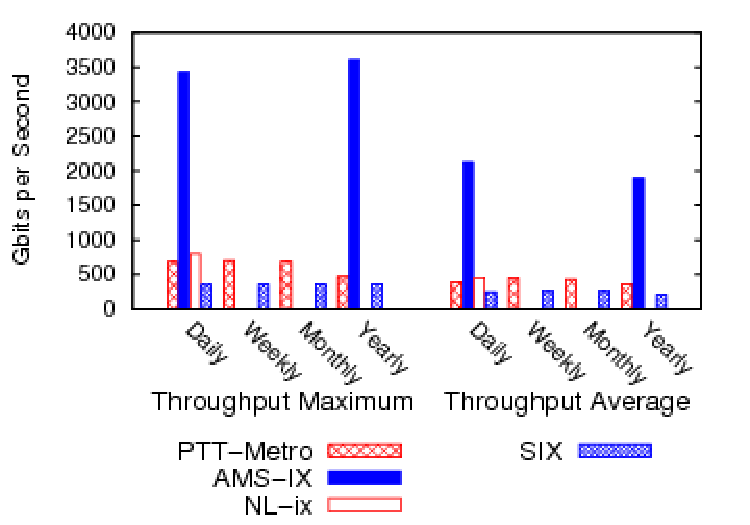
\includegraphics[scale=0.7]{figures/Traffic_Comparison.pdf}
  \label{fig:IXP}
}
\caption{Traffic Comparison}
\end{figure}

%--- Start of Table
\begin{table}[t]
\caption{Traffic comparison between IXPs}            
\scriptsize                                                             
\centering                                                                  
\begin{tabular}{l| l| r r| l}                                        
\hline                                                                      
\textbf{\begin{tabular}[c]{@{}c@{}}Short \\ Name\end{tabular}} & \textbf{Country} & \textbf{\begin{tabular}[c]{@{}c@{}}Throughput \\ Maximum\\ (Gbit/s)\end{tabular}} & \textbf{\begin{tabular}[c]{@{}c@{}}Throughput\\ Average\\ (Gbit/s)\end{tabular}} & \textbf{}
\\\hline
PTT Metro	& Brazil			&678.50		&393.32 	&(1)\\
AMS-IX		& Netherlands		&3429.38	&2120.70   &(2)\\
MSK-IX		& Russia			&1332.63	&751.24	&(3)\\
DE-CIX		& Germany			&3603.10 	&2375.9  	&(4)\\
LINX		& United Kingdom	&2352.13	&1419.26   &(5)\\
NL-ix  		& Europe			&801.14		&456.48  	&(6)\\                                                                        
SIX  		& USA, Canada		&347.84		&250.94  	&(7)\\                                                                        
JPIX  		& Japan				&303.78		&186.89  	&(8)\\                                                                        
\hline       
\multicolumn{5}{l}{\textit{Values updated: 03/25/2015}}\\         
\multicolumn{5}{l}{\textit{(1) http://ptt.br/cgi-bin/all}}\\                           
\multicolumn{5}{l}{\textit{(2) https://ams-ix.net/technical/statistics}}\\                           
\multicolumn{5}{l}{\textit{(3) http://www.msk-ix.ru/network/traffic.html}}\\                           
\multicolumn{5}{l}{\textit{(4) http://www.de-cix.net/about/statistics/}}\\                           
\multicolumn{5}{l}{\textit{(5) https://www.linx.net/pubtools/trafficstats.html}}\\                           
\multicolumn{5}{l}{\textit{(6) https://www.nl-ix.net/network/traffic/}}\\                           
\multicolumn{5}{l}{\textit{(7) http://www.seattleix.net/agg.htm}}\\                  
\multicolumn{5}{l}{\textit{(8) http://www.jpix.ad.jp/en/technical/traffic.html}}                  
\end{tabular}
\label{tab:Traffic1}                               
\end{table}
%--- End of Table

\vspace{1,5cm}

\end{document}
